\pdfminorversion=7
\documentclass[11pt,letterpaper]{article}

\usepackage[margin=0.82in]{geometry}
\usepackage[T1]{fontenc}
\usepackage[utf8]{inputenc}
\usepackage{newtxtext,newtxmath}
\usepackage{amsmath}
\usepackage{array}
\usepackage{booktabs}
\usepackage{float}
\usepackage{graphicx}
\usepackage{xcolor}
\usepackage{tikz}
\usepackage{enumitem}
\usepackage[hidelinks]{hyperref}
\usetikzlibrary{arrows.meta,calc,positioning}

\definecolor{Ink}{HTML}{23201D}
\definecolor{SoftRed}{HTML}{B23B31}
\definecolor{SoftBlue}{HTML}{2F5F9F}
\definecolor{SoftGray}{HTML}{6D6862}
\definecolor{SoftGold}{HTML}{B9842C}
\definecolor{SoftGreen}{HTML}{3F7D5A}
\definecolor{PanelFill}{HTML}{FAF7F1}
\definecolor{SoftBlueFill}{HTML}{EDF3FB}
\definecolor{SoftRedFill}{HTML}{FCF0EE}
\definecolor{SoftGreenFill}{HTML}{EEF7F2}

\hypersetup{
  pdftitle={Wavevis connector assignment: all-four equal X-cell infeasibility and pairwise X-cell result},
  pdfauthor={Wavevis inverse-sheet constraint note},
  pdfsubject={Constraint evidence for contacted connector assignments on a curved overhang}
}

\setlength{\parindent}{0pt}
\setlength{\parskip}{0.52em}
\setlength{\fboxsep}{0.66em}
\renewcommand{\arraystretch}{1.12}
\newcolumntype{Y}[1]{>{\raggedright\arraybackslash}p{#1}}
\setlist[itemize]{leftmargin=1.35em,itemsep=0.15em,topsep=0.2em}
\setlist[enumerate]{leftmargin=1.45em,itemsep=0.15em,topsep=0.2em}
\color{Ink}

\tikzset{
  proofpanel/.style={draw=SoftGray!35,fill=PanelFill,line width=0.55pt,rounded corners=4pt},
  paneltitle/.style={anchor=west,font=\bfseries\small,text=Ink},
  panelsubtitle/.style={anchor=west,font=\scriptsize,text=SoftGray},
  figurecallout/.style={draw=SoftGray!45,fill=white,line width=0.45pt,rounded corners=2pt,align=left,font=\scriptsize,inner sep=4pt},
  redcallout/.style={draw=SoftRed!70,fill=SoftRedFill,line width=0.55pt,rounded corners=2pt,align=left,font=\scriptsize,inner sep=4pt,text=Ink},
  greencallout/.style={draw=SoftGreen!70,fill=SoftGreenFill,line width=0.55pt,rounded corners=2pt,align=left,font=\scriptsize,inner sep=4pt,text=Ink},
  equationbadge/.style={draw=SoftRed!80,fill=SoftRedFill,line width=0.55pt,rounded corners=2pt,align=center,font=\scriptsize,inner sep=4pt,text=SoftRed},
  connectorlabel/.style={font=\scriptsize,inner sep=1.5pt,fill=white,rounded corners=1pt},
  cellbody/.style={draw=Ink,fill=Ink!92,line width=0.8pt,rounded corners=0.6pt},
  centerpt/.style={circle,fill=Ink,inner sep=1.8pt},
  connector/.style={circle,draw=SoftBlue,fill=white,line width=0.85pt,inner sep=2.2pt},
  badconnector/.style={circle,draw=SoftRed,fill=white,line width=0.95pt,inner sep=2.2pt},
  arm/.style={line width=1.15pt,Ink,line cap=round},
  pairarm/.style={line width=1.15pt,SoftGreen,line cap=round},
  badarm/.style={line width=1.15pt,SoftRed,line cap=round},
  guide/.style={line width=0.55pt,SoftGray,dashed},
  softline/.style={line width=0.65pt,SoftGray},
  dim/.style={Latex-Latex,line width=0.55pt,SoftGray},
  note/.style={align=center,font=\small},
  smallnote/.style={align=center,font=\footnotesize}
}

\title{\vspace{-1.5em}Wavevis overhang connector assignment: evidence rejecting all-four-equal X-cells}
\author{Wavevis inverse-sheet constraint note}
\date{June 4, 2026}

\begin{document}
\maketitle
\vspace{-1.2em}

\begin{center}
\fcolorbox{SoftRed}{SoftRed!7}{%
\begin{minipage}{0.93\linewidth}
\textbf{Decision.} Reject the all-four-equal X-cell as a Wavevis overhang mechanism direction. The strict target--one common arm length for all four arms, perpendicular arm pairs, shared connector contact, surface-following links, no gaps, no spikes, no zig-zag, no crossings, and constrained flat-water boundary--was attempted and did not close. The weaker all-four-same-length X-cell with free pair angle also fails for the current sampled overhang when each square cell body stays assigned to its target lattice point. A necessary linear relaxation of that global connector problem has no solution: its least-squares residual norm is \(13.837\), with RMS residual \(0.329\) over \(1764\) interior equal-length equations.

\textbf{Accepted direction.} Use connected pairwise X-cells. The current mechanism keeps the constraints that can be closed: shared connectors, no endpoint gaps, no center drift, surface-near links, and equal/collinear opposite pairs. Perpendicularity and one common all-four length are intentionally relaxed. The resulting pairwise X-cell solve has maximum connector gap \(0\), maximum opposite-pair length spread \(0\), maximum opposite-pair collinearity error \(0^\circ\), and maximum center shift \(0\).
\end{minipage}}
\end{center}

\textbf{Cell-body position definition.} The square prism in the middle of each X-cell has a target location on the sampled overhang. In this proof those square cell-body locations are fixed. The connector points between neighboring cells may be reassigned, but the cell bodies themselves are not allowed to slide to a different lattice.

\textbf{Why this assumption exists.} Allowing the cell bodies to slide is a different mechanism design problem, not a small numerical detail. The current simulator starts from a square grid and samples a target overhang; each square body is assigned to one target grid location so the overhang shape, flat-water boundary, and row/column lattice identity stay defined. If the cell bodies can slide freely, the solver is no longer only assigning shared connectors. It is also remeshing the overhang: cells can bunch, drift, change local spacing, and change which part of the surface each cell represents. That is outside the mechanism contract evaluated here; it is not evidence that the all-four-equal branch works for Wavevis.

\textbf{Claim.} For the current \(44\times44\) sampled Wavevis overhang with those cell-body positions fixed, adjacent cells sharing connector endpoints, and opposite legs forced to remain collinear through each cell, no global assignment can make all four arms of every interior cell have one common length. The impossibility holds even after perpendicularity is removed. A clean connected mechanism becomes available only after the cell is changed to a pairwise X-cell: east/west are one equal collinear pair, north/south are a second equal collinear pair, and the angle and length relation between the two pairs are free.

\textbf{What is proved and what is not.} The algebra below proves two things. First, for any fixed contacted connector points around one cell, all-four equal length requires exact equal-radius and midpoint conditions. Second, for the current Wavevis lattice with the cell-body positions fixed, even allowing the connectors to be reassigned globally cannot satisfy all-four equal length; the necessary linear relaxation is inconsistent. Changing the target parametrization, moving the cell bodies, changing the topology, changing the boundary, or accepting a gap/residual changes the problem rather than rescuing this one. This document rules out the requested all-four-equal X-cell under the current fixed-cell-position, shared-connector overhang contract.

\textbf{Sliding-cell-body answer.} Sliding was tested as the strongest escape route. It does not rescue the all-four-equal branch for this mechanism. If square bodies slide freely, the fixed-position proof alone no longer applies because the problem becomes remeshing. But the finite Wavevis mechanism still has the hard checks that matter: the connector graph must stay shared, ordered, non-overlapping, non-spiking, boundary-preserving, and visually embedded on the overhang. The finite sliding projection found the tradeoff directly: near-equal arms require folding, while clean embedding requires giving up all-four equality. Therefore the simulator rejects all-four-equal X-cells for this overhang contract and uses the pairwise X-cell model.

\textbf{Scope.} A perfectly symmetric flat square grid can satisfy the strict cross constraints, so a universal ``impossible for every surface'' theorem would be false. That exception does not support the Wavevis design target. The current object is a curved overhang with flat-water boundary constraints, shared finite connectors, and no-fold/no-overlap requirements. For that design class, the all-four-equal X-cell is rejected and the accepted mechanism direction is exact shared contact plus pairwise equal opposite bars.

\begin{center}
\begin{tabular}{Y{0.23\linewidth}Y{0.31\linewidth}Y{0.34\linewidth}}
\toprule
Question & Short answer & Reason \\
\midrule
Did the strict equal-arm perpendicular assignment close? & No. & The attempt either left connector gaps or broke the strict cell geometry. \\
Did the all-four-equal X-cell close if the pair angle is free? & No. & A necessary global linear relaxation for the current fixed-cell-position overhang is inconsistent. \\
What should stay hard? & Contact and pairwise cleanliness. & Shared connector endpoints, no visible gaps, no spikes, no zig-zag, surface-near links, flat boundary, and equal collinear opposite pairs. \\
What relaxation worked? & Pairwise X-cells. & East-west may use length \(L_x\); north-south may use length \(L_y\); the included angle \(\theta\) is free. \\
Did sliding cell bodies save all-four equality? & No. & The finite no-fold projection below rejects it for this simulator contract: equality folds the lattice; clean embedding loses equality. \\
\bottomrule
\end{tabular}
\end{center}

\section*{0. Visual map of the proof}

The whole question is which constraints can be kept hard without forcing gaps. The diagrams below show the strict-cell tests and the accepted pairwise X-cell contract.

\begin{center}
\begin{tabular}{Y{0.3\linewidth}Y{0.32\linewidth}Y{0.3\linewidth}}
\toprule
Requested clean cell & Algebraic consequence & What the current overhang does \\
\midrule
Four arms have one common length \(L\). & All four contacted connector points must be the same distance from \(C\). & The current fixed-cell-position global problem fails a stronger linear-relaxation test. \\
Opposite legs are not zig-zagged. & Each opposite connector pair must have midpoint exactly \(C\). & The pairwise X-cell construction enforces this per opposite pair. \\
Two pairs stay perpendicular. & The two through-cell directions must have dot product zero. & This is relaxed; current pair angles vary by as much as \(61.65^\circ\) away from \(90^\circ\). \\
\bottomrule
\end{tabular}
\end{center}

\begin{center}
\fcolorbox{SoftGray!45}{PanelFill}{%
\begin{minipage}{0.93\linewidth}
\textbf{What the two simulator outcomes mean.}
\begin{itemize}
  \item \textbf{All-four equal X-cell:} exact connector contact, no zig-zag legs, and one common length for all four arms, with pair angle free. This is still too constrained for the current fixed-cell-position overhang: a necessary linear system has no solution.
  \item \textbf{Working relaxed constraint:} keep the clean through-cell idea only pairwise. East and west are equal and collinear; north and south are equal and collinear; the two pair lengths and the included angle are allowed to differ. This removes the contradiction while preserving the visual idea of a clean crossed cell.
\end{itemize}
\end{minipage}}
\end{center}

\begin{figure}[H]
\centering
{\setlength{\fboxsep}{0pt}\fcolorbox{SoftGray!45}{white}{
\includegraphics[width=0.98\linewidth]{proofs/figures/constraint-contract-summary.png}}}
\caption{Constraint contract. The rejected Sarrus-like branch requires one common length and a hard right angle. The accepted branch keeps exact shared contact and pairwise equal, collinear opposite arms, while allowing separate pair lengths and a free included angle.}
\end{figure}

\begin{figure}[H]
\centering
{\setlength{\fboxsep}{0pt}\fcolorbox{SoftGray!45}{white}{
\includegraphics[width=0.98\linewidth]{proofs/figures/projection-tradeoff-summary.png}}}
\caption{Finite sliding-cell test. The all-four-equal branch has no clean operating point in the current Wavevis contract: the near-equal-arm result folds the lattice, and the clean embedding result loses equal-arm closure.}
\end{figure}

\begin{figure}[H]
\centering
{\setlength{\fboxsep}{0pt}\fcolorbox{SoftGray!45}{white}{
\includegraphics[width=0.98\linewidth]{proofs/figures/simulator-evidence-plate.png}}}
\caption{Actual Wavevis simulator evidence. The failed all-four branch produces a high-strain, visibly distorted local mechanism. The pairwise branch keeps the shared-contact invariants and is the mechanism direction used for the overhang work.}
\end{figure}

\clearpage

\begin{figure}[H]
\centering
\resizebox{\linewidth}{!}{%
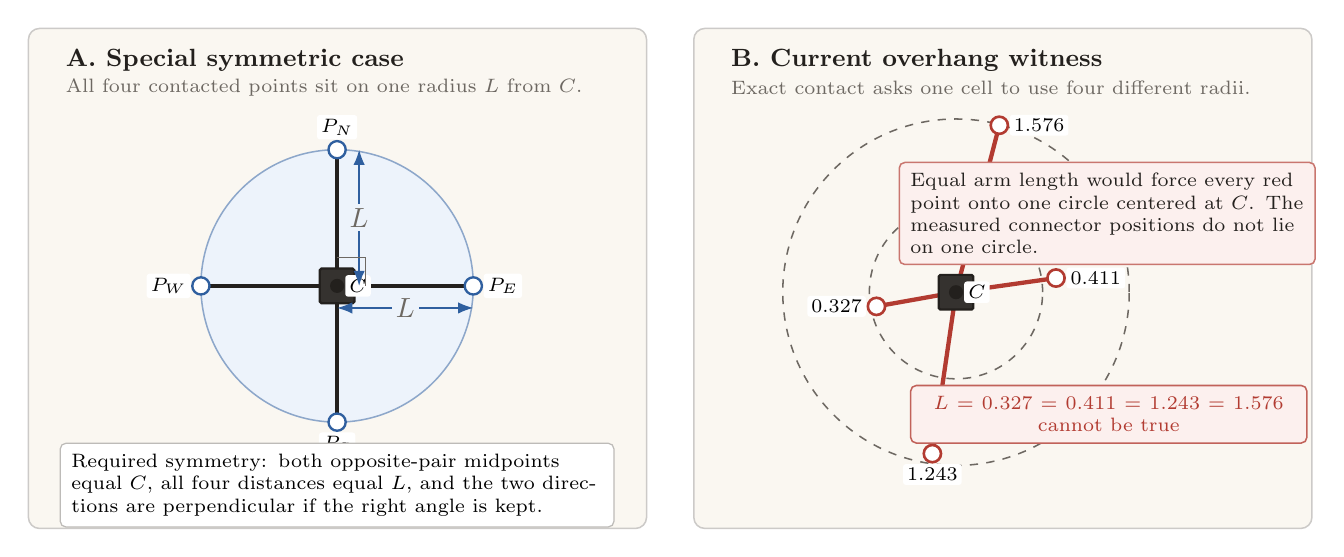
\begin{tikzpicture}[x=1cm,y=1cm]
  \draw[proofpanel] (0,0) rectangle (7.85,6.35);
  \node[paneltitle] at (0.35,5.95) {A. Special symmetric case};
  \node[panelsubtitle] at (0.35,5.6) {All four contacted points sit on one radius \(L\) from \(C\).};

  \coordinate (CA) at (3.92,3.08);
  \coordinate (AE) at (5.65,3.08);
  \coordinate (AW) at (2.19,3.08);
  \coordinate (AN) at (3.92,4.81);
  \coordinate (AS) at (3.92,1.35);
  \draw[draw=SoftBlue!55,fill=SoftBlueFill,line width=0.55pt] (CA) circle (1.73);
  \draw[arm,line width=1.7pt] (AW) -- (AE);
  \draw[arm,line width=1.7pt] (AS) -- (AN);
  \draw[cellbody] ($(CA)+(-0.22,-0.22)$) rectangle ($(CA)+(0.22,0.22)$);
  \node[connector,label={[connectorlabel,anchor=west]right:\(P_E\)}] at (AE) {};
  \node[connector,label={[connectorlabel,anchor=east]left:\(P_W\)}] at (AW) {};
  \node[connector,label={[connectorlabel,anchor=south]above:\(P_N\)}] at (AN) {};
  \node[connector,label={[connectorlabel,anchor=north]below:\(P_S\)}] at (AS) {};
  \node[centerpt,label={[connectorlabel,anchor=west]right:\(C\)}] at (CA) {};
  \draw[dim,draw=SoftBlue] ($(CA)+(0,-0.28)$) -- node[fill=SoftBlueFill,inner sep=1.5pt] {\(L\)} ($(AE)+(0,-0.28)$);
  \draw[dim,draw=SoftBlue] ($(CA)+(0.28,0)$) -- node[fill=SoftBlueFill,inner sep=1.5pt] {\(L\)} ($(AN)+(0.28,0)$);
  \draw[softline] ($(CA)+(0.36,0)$) -- ($(CA)+(0.36,0.36)$) -- ($(CA)+(0,0.36)$);
  \node[figurecallout,text width=6.75cm] at (3.92,0.55) {Required symmetry: both opposite-pair midpoints equal \(C\), all four distances equal \(L\), and the two directions are perpendicular if the right angle is kept.};

  \draw[proofpanel] (8.45,0) rectangle (16.3,6.35);
  \node[paneltitle] at (8.8,5.95) {B. Current overhang witness};
  \node[panelsubtitle] at (8.8,5.6) {Exact contact asks one cell to use four different radii.};

  \coordinate (CB) at (11.78,3.0);
  \coordinate (BE) at (13.05,3.18);
  \coordinate (BW) at (10.77,2.82);
  \coordinate (BN) at (12.33,5.12);
  \coordinate (BS) at (11.48,0.95);
  \draw[guide] (CB) circle (1.1);
  \draw[guide] (CB) circle (2.2);
  \draw[badarm,line width=1.55pt] (CB) -- (BE);
  \draw[badarm,line width=1.55pt] (CB) -- (BW);
  \draw[badarm,line width=1.55pt] (CB) -- (BN);
  \draw[badarm,line width=1.55pt] (CB) -- (BS);
  \draw[cellbody] ($(CB)+(-0.22,-0.22)$) rectangle ($(CB)+(0.22,0.22)$);
  \node[badconnector,label={[connectorlabel,anchor=west]right:0.411}] at (BE) {};
  \node[badconnector,label={[connectorlabel,anchor=east]left:0.327}] at (BW) {};
  \node[badconnector,label={[connectorlabel,anchor=west]right:1.576}] at (BN) {};
  \node[badconnector,label={[connectorlabel,anchor=north]below:1.243}] at (BS) {};
  \node[centerpt,label={[connectorlabel,anchor=west]right:\(C\)}] at (CB) {};
  \node[equationbadge,text width=4.75cm] at (13.72,1.45) {\(L=0.327=0.411=1.243=1.576\)\\cannot be true};
  \node[redcallout,text width=5.0cm] at (13.7,4.0) {Equal arm length would force every red point onto one circle centered at \(C\). The measured connector positions do not lie on one circle.};
\end{tikzpicture}}
\caption{Equal-radius obstruction. Panel A shows the special symmetric geometry required by one common arm length. Panel B shows a current Wavevis witness cell: exact connector contact gives four different center-to-connector distances, so no single \(L\) can satisfy all four arms.}
\end{figure}

\clearpage

\begin{figure}[H]
\centering
\resizebox{\linewidth}{!}{%
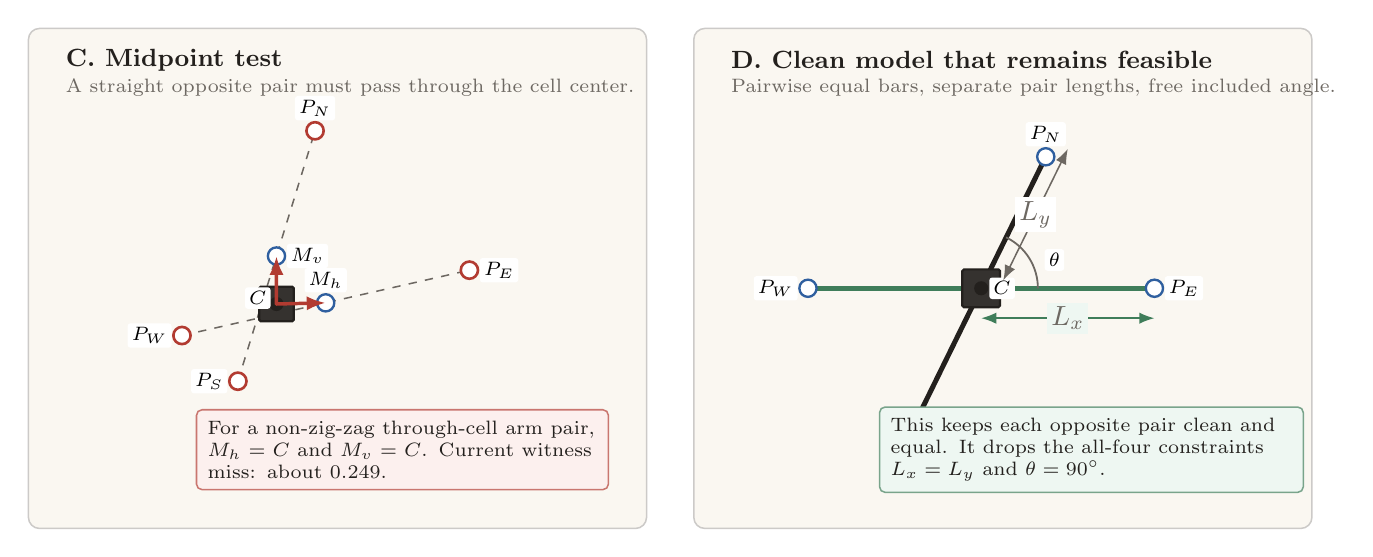
\begin{tikzpicture}[x=1cm,y=1cm]
  \draw[proofpanel] (0,0) rectangle (7.85,6.35);
  \node[paneltitle] at (0.35,5.95) {C. Midpoint test};
  \node[panelsubtitle] at (0.35,5.6) {A straight opposite pair must pass through the cell center.};

  \coordinate (CC) at (3.15,2.85);
  \coordinate (CE) at (5.6,3.28);
  \coordinate (CW) at (1.95,2.45);
  \coordinate (CN) at (3.64,5.05);
  \coordinate (CS) at (2.66,1.87);
  \coordinate (CMh) at ($(CE)!0.5!(CW)$);
  \coordinate (CMv) at ($(CN)!0.5!(CS)$);
  \draw[guide] (CW) -- (CE);
  \draw[guide] (CS) -- (CN);
  \draw[cellbody] ($(CC)+(-0.22,-0.22)$) rectangle ($(CC)+(0.22,0.22)$);
  \node[centerpt,label={[connectorlabel,anchor=south east]below left:\(C\)}] at (CC) {};
  \node[badconnector,label={[connectorlabel,anchor=west]right:\(P_E\)}] at (CE) {};
  \node[badconnector,label={[connectorlabel,anchor=east]left:\(P_W\)}] at (CW) {};
  \node[badconnector,label={[connectorlabel,anchor=south]above:\(P_N\)}] at (CN) {};
  \node[badconnector,label={[connectorlabel,anchor=east]left:\(P_S\)}] at (CS) {};
  \node[connector,label={[connectorlabel,anchor=south]above:\(M_h\)}] at (CMh) {};
  \node[connector,label={[connectorlabel,anchor=west]right:\(M_v\)}] at (CMv) {};
  \draw[badarm,line width=1.25pt,-{Latex[length=2.4mm]}] (CC) -- (CMh);
  \draw[badarm,line width=1.25pt,-{Latex[length=2.4mm]}] (CC) -- (CMv);
  \node[redcallout,text width=4.95cm] at (4.75,1.0) {For a non-zig-zag through-cell arm pair, \(M_h=C\) and \(M_v=C\). Current witness miss: about \(0.249\).};

  \draw[proofpanel] (8.45,0) rectangle (16.3,6.35);
  \node[paneltitle] at (8.8,5.95) {D. Clean model that remains feasible};
  \node[panelsubtitle] at (8.8,5.6) {Pairwise equal bars, separate pair lengths, free included angle.};

  \coordinate (CD) at (12.1,3.05);
  \coordinate (DE) at (14.3,3.05);
  \coordinate (DW) at (9.9,3.05);
  \coordinate (DN) at (12.92,4.72);
  \coordinate (DS) at (11.28,1.38);
  \draw[pairarm,line width=1.8pt] (DW) -- (DE);
  \draw[arm,line width=1.8pt] (DS) -- (DN);
  \draw[cellbody] ($(CD)+(-0.24,-0.24)$) rectangle ($(CD)+(0.24,0.24)$);
  \node[connector,label={[connectorlabel,anchor=west]right:\(P_E\)}] at (DE) {};
  \node[connector,label={[connectorlabel,anchor=east]left:\(P_W\)}] at (DW) {};
  \node[connector,label={[connectorlabel,anchor=south]above:\(P_N\)}] at (DN) {};
  \node[connector,label={[connectorlabel,anchor=north]below:\(P_S\)}] at (DS) {};
  \node[centerpt,label={[connectorlabel,anchor=west]right:\(C\)}] at (CD) {};
  \draw[dim,draw=SoftGreen] ($(CD)+(0,-0.38)$) -- node[fill=SoftGreenFill,inner sep=1.5pt] {\(L_x\)} ($(DE)+(0,-0.38)$);
  \draw[dim,draw=SoftGray] ($(CD)+(0.28,0.1)$) -- node[fill=white,inner sep=1.5pt] {\(L_y\)} ($(DN)+(0.28,0.1)$);
  \draw[softline] ($(CD)+(0.72,0)$) arc[start angle=0,end angle=64,radius=0.72];
  \node[connectorlabel] at ($(CD)+(0.93,0.36)$) {\(\theta\)};
  \node[greencallout,text width=5.1cm] at (13.5,1.0) {This keeps each opposite pair clean and equal. It drops the all-four constraints \(L_x=L_y\) and \(\theta=90^\circ\).};
\end{tikzpicture}}
\caption{Midpoint obstruction and viable relaxation. Panel C shows the separate through-center condition needed to avoid zig-zag legs. Panel D shows the first clean model with enough freedom for exact contact on the curved overhang: opposite legs stay collinear and equal within each pair, but the two pair lengths and included angle are independent.}
\end{figure}

\clearpage

\section*{1. Definitions}

Consider one cell with center point \(C \in \mathbb{R}^3\). Let the four contacted connector points assigned to that cell be
\[
P_E,\quad P_W,\quad P_N,\quad P_S.
\]
``Contact'' means the visible arm endpoint equals the prescribed connector point. Therefore the four arm vectors are
\[
e=P_E-C,\quad w=P_W-C,\quad n=P_N-C,\quad s=P_S-C.
\]

The phrase ``avoid weird zig-zag legs'' is treated as a hard visual/kinematic constraint:
\[
\text{opposite arms must be straight through the cell center.}
\]
That means the east and west arms lie on one line through \(C\), and the north and south arms lie on another line through \(C\).

\section*{2. Hard equal-length cross with perpendicular pairs}

This is the strongest requested model. It requires unit directions \(u\) and \(v\), one common half-arm length \(L>0\), and perpendicular arm-pairs:
\[
P_E=C+Lu,\quad P_W=C-Lu,\quad P_N=C+Lv,\quad P_S=C-Lv,\quad u\cdot v=0.
\]

\textbf{Necessary conditions.} If these equations hold, then:
\[
\frac{P_E+P_W}{2}=C,\qquad \frac{P_N+P_S}{2}=C
\tag{1}
\]
\[
\|P_E-C\|=\|P_W-C\|=\|P_N-C\|=\|P_S-C\|=L
\tag{2}
\]
\[
(P_E-C)\cdot(P_N-C)=0.
\tag{3}
\]

\textbf{Why.} Equation (1) follows because \(C+Lu\) and \(C-Lu\) average to \(C\), and similarly for \(v\). Equation (2) follows because every vector is either \(Lu\), \(-Lu\), \(Lv\), or \(-Lv\), all with norm \(L\). Equation (3) is perpendicularity.

\textbf{Sufficient conditions.} Conversely, if (1), (2), and (3) hold, then define
\[
u=\frac{P_E-C}{L},\qquad v=\frac{P_N-C}{L}.
\]
The conditions reconstruct the exact perpendicular equal-length cross. So (1)--(3) are not just nice-to-have checks; they are the exact algebraic test.

\textbf{Conclusion.} If any one of (1), (2), or (3) fails for the contacted connector points of a cell, then exact contact and this clean equal-length perpendicular cross are kinematically impossible for that cell. No rotation of the cross, choice of local axes, or numerical solve can remove that contradiction while the connector points and cell center remain fixed.

\section*{3. Equal-length cross without requiring perpendicular pairs}

Now remove the perpendicular condition. This is weaker:
\[
P_E=C+Lu,\quad P_W=C-Lu,\quad P_N=C+Lv,\quad P_S=C-Lv
\]
where \(u\) and \(v\) do not have to be perpendicular.

The exact necessary and sufficient conditions become only:
\[
\frac{P_E+P_W}{2}=C,\qquad \frac{P_N+P_S}{2}=C
\tag{4}
\]
\[
\|P_E-C\|=\|P_W-C\|=\|P_N-C\|=\|P_S-C\|=L.
\tag{5}
\]

Perpendicularity is gone, but the common radius \(L\) remains. Therefore all four contacted connector points must still lie on one sphere centered at \(C\), and opposite pairs must still be symmetric through \(C\).

\textbf{Conclusion.} Dropping the right angle does not solve the main problem. If the four contacted connector distances from \(C\) are unequal, then no equal-length through-cross can contact them, even if the two arm-pairs are allowed to meet at any angle. The all-four equal-length condition alone forces all four contacted points onto one sphere centered at \(C\).

\section*{4. Numerical witness from the strict all-constraints attempt}

For the all-constraints attempt on the current Wavevis overhang, before the accepted pairwise X-cell reassignment, the contacted connector geometry was evaluated from the local model on June 4, 2026. One witness cell gave the following distances from its center to its four contacted connector points:

\begin{center}
\begin{tabular}{lll}
\toprule
Cell & Connector edge & Distance from cell center \\
\midrule
\(n\)-10-26 & \(e\)-h-10-25 & 0.411 \\
\(n\)-10-26 & \(e\)-h-10-26 & 0.327 \\
\(n\)-10-26 & \(e\)-v-9-26  & 1.576 \\
\(n\)-10-26 & \(e\)-v-10-26 & 1.243 \\
\bottomrule
\end{tabular}
\end{center}

The spread between the shortest and longest required contacted arm lengths is
\[
1.576-0.327=1.249.
\]

If all four arms had one common length \(L\), then the same cell would require
\[
L=0.411,\quad L=0.327,\quad L=1.576,\quad L=1.243
\]
simultaneously. That is a contradiction. Therefore, for this cell, exact connector contact and equal length of all four arms cannot both be true.

For this fixed contacted connector assignment, that contradiction rules out both strict interpretations:
\begin{itemize}
  \item The perpendicular equal-length cross cannot fit these four fixed contacted points, because it requires equal distances.
  \item The non-perpendicular equal-length cross with one common all-four length also cannot fit these four fixed contacted points, because it still requires equal distances.
\end{itemize}
This local witness is useful but not enough by itself, because it assumes those four connector points were already fixed. The next section removes that loophole for the current fixed-cell-position lattice by allowing the shared connectors to be reassigned globally and then proving that even the necessary relaxed equations are inconsistent.

A second independent check shows the through-center symmetry condition was also violated in that strict contacted layout. For cell \(n\)-8-21, the midpoint disagreement between the opposite-pair connector midpoints and the cell center was approximately
\[
0.249.
\]
For any exact through-line pair, that value must be exactly zero:
\[
\frac{P_E+P_W}{2}=C,\qquad \frac{P_N+P_S}{2}=C.
\]
So that strict contacted layout also fails the required midpoint condition for a clean through-cell model.

\section*{5. Global fixed-cell-position infeasibility certificate}

Now allow the contacted connectors to be reassigned globally, but keep the square cell bodies at their target locations on the sampled overhang. This is the question that matters for the simulator: can a better connector assignment make every cell an all-four-equal X-cell while preserving exact shared connector contact and non-zig-zag opposite pairs?

Let \(H_{i,j}\) be the horizontal connector shared by cells \((i,j)\) and \((i,j+1)\), and let \(V_{i,j}\) be the vertical connector shared by cells \((i,j)\) and \((i+1,j)\). Let the fixed cell center be \(C_{i,j}\).

Opposite legs collinear and equal as a pair force the connector midpoint equations
\[
H_{i,j-1}+H_{i,j}=2C_{i,j},\qquad
V_{i-1,j}+V_{i,j}=2C_{i,j}.
\tag{8}
\]
Therefore, every horizontal connector in row \(i\) is determined by one row seed vector \(p_i\), and every vertical connector in column \(j\) is determined by one column seed vector \(q_j\):
\[
H_{i,j}=(-1)^j p_i + a_{i,j},\qquad
V_{i,j}=(-1)^i q_j + b_{i,j},
\tag{9}
\]
where \(a_{i,j}\) and \(b_{i,j}\) are known vectors computed only from the fixed cell-body positions \(C_{i,j}\).

All four arms having one common length in each interior cell then requires
\[
\|H_{i,j}-C_{i,j}\|^2=\|V_{i,j}-C_{i,j}\|^2.
\tag{10}
\]
After substituting (9), each equation has the form
\[
\|p_i\|^2 + 2p_i\cdot \alpha_{i,j} + \beta_{i,j}
-\|q_j\|^2 - 2q_j\cdot \gamma_{i,j} - \delta_{i,j}=0.
\tag{11}
\]
This is nonlinear only because of the squared seed lengths \(\|p_i\|^2\) and \(\|q_j\|^2\). Introduce relaxed scalar variables
\[
s_i=\|p_i\|^2,\qquad t_j=\|q_j\|^2
\]
but do not enforce that relation. This makes a necessary linear system
\[
Ax=b.
\tag{12}
\]
Every true all-four-equal X-cell solution would produce a solution of this relaxed linear system. Therefore, if (12) has no solution, the original nonlinear mechanism is impossible.

For the current \(44\times44\) Wavevis overhang, the interior cells give \(42\times42=1764\) equal-length equations. The linear relaxation has \(352\) variables: \(p_i\in\mathbb{R}^3\) and \(s_i\) for each of \(44\) rows, plus \(q_j\in\mathbb{R}^3\) and \(t_j\) for each of \(44\) columns.

\begin{center}
\begin{tabular}{Y{0.45\linewidth}Y{0.32\linewidth}}
\toprule
Linear-relaxation check & Value \\
\midrule
Equations & \(1764\) \\
Variables & \(352\) \\
Rank of \(A\) & \(269\) \\
Least-squares residual norm \(\|Ax^\ast-b\|\) & \(13.837\) \\
Residual RMS & \(0.329\) \\
Maximum absolute residual & \(1.432\) \\
\bottomrule
\end{tabular}
\end{center}

The nonzero least-squares residual means \(b\) is not in the column space of \(A\). Equivalently, the residual vector
\[
y=Ax^\ast-b
\]
is a numerical left-null certificate:
\[
A^Ty\approx 0,\qquad y^Tb=-191.453\neq 0.
\tag{13}
\]
The measured value was \(\|A^Ty\|=7.94\times10^{-7}\), while \(|y^Tb|=191.453\). So the relaxed linear system is inconsistent by a large margin compared with numerical roundoff.

\textbf{Conclusion.} For the current sampled overhang with cell-body positions fixed, exact shared connectors, opposite-pair collinearity, and all-four equal arm length cannot all hold, even when the pair angle is completely free. This is stronger than the local witness above: it rules out a better global connector assignment under the same fixed-cell-position lattice contract.

\textbf{Remaining escape routes.} The proof does not rule out changing the problem itself: moving cell bodies away from the sampled target, changing the target parametrization, changing the grid topology, relaxing exact contact, allowing non-collinear/zig-zag legs, or allowing the flat-water boundary to move. It rules out the requested all-four-equal X-cell for the current fixed-cell-position Wavevis overhang.

\section*{6. What relaxed model is actually feasible}

A clean contacted cell can exist if the two opposite arm-pairs are treated as two separate bars:
\[
P_E=C+L_xu,\quad P_W=C-L_xu
\]
\[
P_N=C+L_yv,\quad P_S=C-L_yv
\]
where:
\[
L_x \neq L_y \quad \text{is allowed}
\]
and
\[
u\cdot v \neq 0 \quad \text{is allowed.}
\]

This model still preserves the important clean visual constraint:
\begin{itemize}
  \item east and west are collinear and equal to each other;
  \item north and south are collinear and equal to each other;
  \item the cell looks like two straight bars crossing at the body, not like four random zig-zag spokes.
\end{itemize}

The exact algebraic test for this relaxed model is:
\[
\frac{P_E+P_W}{2}=C,\qquad \|P_E-C\|=\|P_W-C\|=L_x
\tag{6}
\]
\[
\frac{P_N+P_S}{2}=C,\qquad \|P_N-C\|=\|P_S-C\|=L_y.
\tag{7}
\]

No condition requires \(L_x=L_y\), and no condition requires \(u\cdot v=0\).

\textbf{Interpretation.} This is the first clean-contact model with enough freedom to follow a curved overhang without forcing visible zig-zag arms. It preserves pairwise straightness, but gives up the single common length and the fixed right angle. In practice, exact contact must be solved with this pairwise model: the east-west contact pair and the north-south contact pair each need their own length, and the included angle between the pairs must be free.

If the pairwise midpoint equations in (6) and (7) are also impossible for a chosen fixed center, then the remaining choices are mechanical, not cosmetic: move the center, move the contacted connector assignment, allow a contact residual/gap, or allow a zig-zag/non-collinear leg. A smooth renderer cannot make an incompatible set of endpoint constraints true.

\begin{center}
\begin{tabular}{Y{0.34\linewidth}Y{0.18\linewidth}Y{0.34\linewidth}}
\toprule
Current pairwise X-cell check & Value & Interpretation \\
\midrule
Maximum shared connector endpoint gap & \(0\) & Adjacent cells meet at the same connector point; no visible gap is being hidden. \\
Maximum opposite-pair length spread & \(0\) & East/west match each other and north/south match each other. \\
Maximum opposite-pair collinearity error & \(0^\circ\) & Opposite legs form straight through-cell pairs instead of zig-zag spokes. \\
Maximum center shift & \(0\) & The solve does not cheat by moving cell bodies off the sampled surface. \\
Maximum arm surface residual & \(0.111\) & Links remain close to the surface field instead of becoming random vertical spikes. \\
All-four length spread & \(1.218\) & Expected: \(L_x\) and \(L_y\) are allowed to differ. \\
Pair-angle error from \(90^\circ\) & \(61.65^\circ\) & Expected: the included angle is allowed to change. \\
\bottomrule
\end{tabular}
\end{center}

\section*{7. Sliding-cell-body attempt: why it still failed}

Let \(r(s,t)\) describe the target overhang surface in whatever coordinates the cell-body lattice finally uses. For a small all-four-equal X-cell, the two through-cell arm directions are the local coordinate directions. If the half-step is \(h\), then to first order the four connector distances are
\[
h\|r_s\|,\qquad h\|r_t\|.
\tag{14}
\]
One common arm length therefore asks for
\[
\|r_s\|=\|r_t\|.
\tag{15}
\]
If the two arm pairs must also be perpendicular, the local condition adds
\[
r_s\cdot r_t=0.
\tag{16}
\]
Equations (15) and (16) are the metric conditions for a conformal coordinate net. This is why the sliding-cell version is not killed by the fixed-cell-position certificate: the sliding version is allowed to change \(s,t\), so it is allowed to search for a better coordinate net on the same surface.

\textbf{Why this does not reopen the design.} The continuum observation only says why flat or specially remeshed cases can exist. It does not solve the finite mechanism Alan is trying to build. A Wavevis mechanism is not allowed to remesh by folding, overlapping, losing the flat-water boundary, changing connector order, creating gaps, or producing spikes. The sliding branch must therefore pass finite embedding checks, not only local equal-scale equations.

\textbf{Finite projection test.} A sliding-cell projection was added after the fixed-position proof. The projection moved cell-body centers and shared connectors, then measured whether the all-four equal-arm condition could coexist with two embedding checks:
\begin{itemize}
  \item a shared connector for neighboring cells must stay inside the neighbor corridor instead of jumping behind either cell;
  \item the ordered center quads must not collapse or flip.
\end{itemize}

\begin{center}
\begin{tabular}{Y{0.31\linewidth}Y{0.18\linewidth}Y{0.18\linewidth}Y{0.18\linewidth}}
\toprule
Sliding attempt & All-four spread & Corridor / fold result & Interpretation \\
\midrule
Equal-arm first & \(0.0022\) & \(18\) outside-corridor connectors, \(4\) flipped quads, minimum quad area ratio \(0.0656\) & Numerically equal, geometrically folded. \\
Mild no-fold corridor & \(0.2275\) & \(324\) outside-corridor connectors, \(16\) flipped quads & Still folded and no longer equal-arm. \\
Strong no-fold corridor & \(0.1854\) & \(0\) outside connectors, \(45\) flipped quads & Connector corridor improves, center lattice still flips. \\
Locked neighbor corridor & \(0.3629\) & \(0\) outside connectors, \(0\) flipped quads & Clean embedding check passes, but equal-arm closure fails. \\
\bottomrule
\end{tabular}
\end{center}

All values are in normalized grid units. The equal-arm-first result explains the bad visual render: it achieves nearly equal arms only by folding the lattice and placing connectors outside the local neighbor corridor. Once the no-fold corridor is enforced strongly enough to remove outside connectors and flipped center quads, the all-four arm-length spread rises to \(0.3629\), far above the \(0.0022\) equal-arm residual and large enough to be visible.

\textbf{What this rules out.} This rejects the all-four-equal X-cell for the current Wavevis overhang mechanism: same sampled overhang, preserved flat boundary, shared connectors, no gaps, no spikes, no visible lattice folding, and all four arms equal in each cell. Under those checks, the sliding-cell branch does not produce a valid mechanism.

\textbf{Decision from the sliding test.} Do not keep iterating on all-four-equal X-cells for Wavevis overhangs. The current finite projection gives the opposite engineering signal: equal arms are obtained by folding; clean embedding is obtained by giving up equal arms. The next mechanism direction is the pairwise opposite-equal X-cell.

\section*{8. Engineering conclusion}

In the implementation that actually closes the current fixed-cell-position Wavevis overhang, exact connector contact and a clean visible mechanism become compatible by relaxing the constraints in the correct order:

\begin{enumerate}
  \item Keep exact connector contact if contact is physically required.
  \item Keep opposite-pair collinearity if avoiding zig-zag legs is visually and mechanically required.
  \item Allow the east-west pair length \(L_x\) to differ from the north-south pair length \(L_y\).
  \item Allow the two pair directions to meet at a non-right angle.
\end{enumerate}

\textbf{Constraint that must be removed:} one common half-arm length for all four arms. This is not merely a failed visual attempt; the global fixed-cell-position linear-relaxation certificate rules it out for fixed cell bodies, and the sliding-cell projection shows the same constraint is not usable once no-fold/no-overlap checks are restored. If perpendicularity is also kept hard, it must be removed as well.

\textbf{Therefore for the current fixed-position solver:} with exact contact and no zig-zag legs as hard constraints, the feasible mechanism is a two-bar crossed cell with pairwise equal opposite legs, separate pair lengths, and a free included angle.

\textbf{Therefore for the sliding-cell branch:} do not use it in the current simulator or as the working mechanism direction. It failed the finite mechanism checks that matter. The all-four-equal constraint remains rejected for Wavevis overhangs; proceed with pairwise opposite-equal X-cells.

\end{document}
